\documentclass[1p]{elsarticle_modified}
%\bibliographystyle{elsarticle-num}

%\usepackage[colorlinks]{hyperref}
%\usepackage{abbrmath_seonhwa} %\Abb, \Ascr, \Acal ,\Abf, \Afrak
\usepackage{amsfonts}
\usepackage{amssymb}
\usepackage{amsmath}
\usepackage{amsthm}
\usepackage{scalefnt}
\usepackage{amsbsy}
\usepackage{kotex}
\usepackage{caption}
\usepackage{subfig}
\usepackage{color}
\usepackage{graphicx}
\usepackage{xcolor} %% white, black, red, green, blue, cyan, magenta, yellow
\usepackage{float}
\usepackage{setspace}
\usepackage{hyperref}

\usepackage{tikz}
\usetikzlibrary{arrows}

\usepackage{multirow}
\usepackage{array} % fixed length table
\usepackage{hhline}

%%%%%%%%%%%%%%%%%%%%%
\makeatletter
\renewcommand*\env@matrix[1][\arraystretch]{%
	\edef\arraystretch{#1}%
	\hskip -\arraycolsep
	\let\@ifnextchar\new@ifnextchar
	\array{*\c@MaxMatrixCols c}}
\makeatother %https://tex.stackexchange.com/questions/14071/how-can-i-increase-the-line-spacing-in-a-matrix
%%%%%%%%%%%%%%%

\usepackage[normalem]{ulem}

\newcommand{\msout}[1]{\ifmmode\text{\sout{\ensuremath{#1}}}\else\sout{#1}\fi}
%SOURCE: \msout is \stkout macro in https://tex.stackexchange.com/questions/20609/strikeout-in-math-mode

\newcommand{\cancel}[1]{
	\ifmmode
	{\color{red}\msout{#1}}
	\else
	{\color{red}\sout{#1}}
	\fi
}

\newcommand{\add}[1]{
	{\color{blue}\uwave{#1}}
}

\newcommand{\replace}[2]{
	\ifmmode
	{\color{red}\msout{#1}}{\color{blue}\uwave{#2}}
	\else
	{\color{red}\sout{#1}}{\color{blue}\uwave{#2}}
	\fi
}

\newcommand{\Sol}{\mathcal{S}} %segment
\newcommand{\D}{D} %diagram
\newcommand{\A}{\mathcal{A}} %arc


%%%%%%%%%%%%%%%%%%%%%%%%%%%%%5 test

\def\sl{\operatorname{\textup{SL}}(2,\Cbb)}
\def\psl{\operatorname{\textup{PSL}}(2,\Cbb)}
\def\quan{\mkern 1mu \triangleright \mkern 1mu}

\theoremstyle{definition}
\newtheorem{thm}{Theorem}[section]
\newtheorem{prop}[thm]{Proposition}
\newtheorem{lem}[thm]{Lemma}
\newtheorem{ques}[thm]{Question}
\newtheorem{cor}[thm]{Corollary}
\newtheorem{defn}[thm]{Definition}
\newtheorem{exam}[thm]{Example}
\newtheorem{rmk}[thm]{Remark}
\newtheorem{alg}[thm]{Algorithm}

\newcommand{\I}{\sqrt{-1}}
\begin{document}

%\begin{frontmatter}
%
%\title{Boundary parabolic representations of knots up to 8 crossings}
%
%%% Group authors per affiliation:
%\author{Yunhi Cho} 
%\address{Department of Mathematics, University of Seoul, Seoul, Korea}
%\ead{yhcho@uos.ac.kr}
%
%
%\author{Seonhwa Kim} %\fnref{s_kim}}
%\address{Center for Geometry and Physics, Institute for Basic Science, Pohang, 37673, Korea}
%\ead{ryeona17@ibs.re.kr}
%
%\author{Hyuk Kim}
%\address{Department of Mathematical Sciences, Seoul National University, Seoul 08826, Korea}
%\ead{hyukkim@snu.ac.kr}
%
%\author{Seokbeom Yoon}
%\address{Department of Mathematical Sciences, Seoul National University, Seoul, 08826,  Korea}
%\ead{sbyoon15@snu.ac.kr}
%
%\begin{abstract}
%We find all boundary parabolic representation of knots up to 8 crossings.
%
%\end{abstract}
%\begin{keyword}
%    \MSC[2010] 57M25 
%\end{keyword}
%
%\end{frontmatter}

%\linenumbers
%\tableofcontents
%
\newcommand\colored[1]{\textcolor{white}{\rule[-0.35ex]{0.8em}{1.4ex}}\kern-0.8em\color{red} #1}%
%\newcommand\colored[1]{\textcolor{white}{ #1}\kern-2.17ex	\textcolor{white}{ #1}\kern-1.81ex	\textcolor{white}{ #1}\kern-2.15ex\color{red}#1	}

{\Large $\underline{12a_{0845}~(K12a_{0845})}$}

\setlength{\tabcolsep}{10pt}
\renewcommand{\arraystretch}{1.6}
\vspace{1cm}\begin{tabular}{m{100pt}>{\centering\arraybackslash}m{274pt}}
\multirow{5}{120pt}{
	\centering
	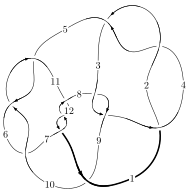
\includegraphics[width=112pt]{../../../GIT/diagram.site/Diagrams/png/1646_12a_0845.png}\\
\ \ \ A knot diagram\footnotemark}&
\allowdisplaybreaks
\textbf{Linearized knot diagam} \\
\cline{2-2}
 &
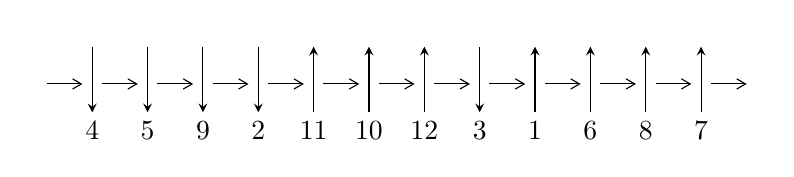
\begin{tikzpicture}[x=20pt, y=17pt]
	% nodes
	\node (C0) at (0, 0) {};
	\node (C1) at (1, 0) {};
	\node (C1U) at (1, +1) {};
	\node (C1D) at (1, -1) {4};

	\node (C2) at (2, 0) {};
	\node (C2U) at (2, +1) {};
	\node (C2D) at (2, -1) {5};

	\node (C3) at (3, 0) {};
	\node (C3U) at (3, +1) {};
	\node (C3D) at (3, -1) {9};

	\node (C4) at (4, 0) {};
	\node (C4U) at (4, +1) {};
	\node (C4D) at (4, -1) {2};

	\node (C5) at (5, 0) {};
	\node (C5U) at (5, +1) {};
	\node (C5D) at (5, -1) {11};

	\node (C6) at (6, 0) {};
	\node (C6U) at (6, +1) {};
	\node (C6D) at (6, -1) {10};

	\node (C7) at (7, 0) {};
	\node (C7U) at (7, +1) {};
	\node (C7D) at (7, -1) {12};

	\node (C8) at (8, 0) {};
	\node (C8U) at (8, +1) {};
	\node (C8D) at (8, -1) {3};

	\node (C9) at (9, 0) {};
	\node (C9U) at (9, +1) {};
	\node (C9D) at (9, -1) {1};

	\node (C10) at (10, 0) {};
	\node (C10U) at (10, +1) {};
	\node (C10D) at (10, -1) {6};

	\node (C11) at (11, 0) {};
	\node (C11U) at (11, +1) {};
	\node (C11D) at (11, -1) {8};

	\node (C12) at (12, 0) {};
	\node (C12U) at (12, +1) {};
	\node (C12D) at (12, -1) {7};
	\node (C13) at (13, 0) {};

	% arrows
	\draw[->,>={angle 60}]
	(C0) edge (C1) (C1) edge (C2) (C2) edge (C3) (C3) edge (C4) (C4) edge (C5) (C5) edge (C6) (C6) edge (C7) (C7) edge (C8) (C8) edge (C9) (C9) edge (C10) (C10) edge (C11) (C11) edge (C12) (C12) edge (C13) ;	\draw[->,>=stealth]
	(C1U) edge (C1D) (C2U) edge (C2D) (C3U) edge (C3D) (C4U) edge (C4D) (C5D) edge (C5U) (C6D) edge (C6U) (C7D) edge (C7U) (C8U) edge (C8D) (C9D) edge (C9U) (C10D) edge (C10U) (C11D) edge (C11U) (C12D) edge (C12U) ;
	\end{tikzpicture} \\
\hhline{~~} \\& 
\textbf{Solving Sequence} \\ \cline{2-2} 
 &
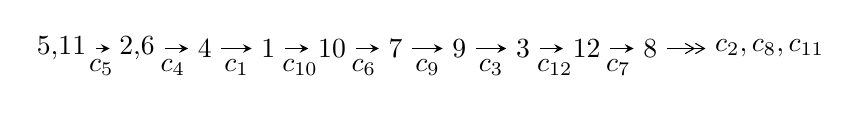
\begin{tikzpicture}[x=23pt, y=7pt]
	% node
	\node (A0) at (-1/8, 0) {5,11};
	\node (A1) at (17/16, 0) {2,6};
	\node (A2) at (17/8, 0) {4};
	\node (A3) at (25/8, 0) {1};
	\node (A4) at (33/8, 0) {10};
	\node (A5) at (41/8, 0) {7};
	\node (A6) at (49/8, 0) {9};
	\node (A7) at (57/8, 0) {3};
	\node (A8) at (65/8, 0) {12};
	\node (A9) at (73/8, 0) {8};
	\node (C1) at (1/2, -1) {$c_{5}$};
	\node (C2) at (13/8, -1) {$c_{4}$};
	\node (C3) at (21/8, -1) {$c_{1}$};
	\node (C4) at (29/8, -1) {$c_{10}$};
	\node (C5) at (37/8, -1) {$c_{6}$};
	\node (C6) at (45/8, -1) {$c_{9}$};
	\node (C7) at (53/8, -1) {$c_{3}$};
	\node (C8) at (61/8, -1) {$c_{12}$};
	\node (C9) at (69/8, -1) {$c_{7}$};
	\node (A10) at (11, 0) {$c_{2},c_{8},c_{11}$};

	% edge
	\draw[->,>=stealth]	
	(A0) edge (A1) (A1) edge (A2) (A2) edge (A3) (A3) edge (A4) (A4) edge (A5) (A5) edge (A6) (A6) edge (A7) (A7) edge (A8) (A8) edge (A9) ;
	\draw[->>,>={angle 60}]	
	(A9) edge (A10);
\end{tikzpicture} \\ 

\end{tabular} \\

\footnotetext{
The image of knot diagram is generated by the software ``\textbf{Draw programme}" developed by Andrew Bartholomew(\url{http://www.layer8.co.uk/maths/draw/index.htm\#Running-draw}), where we modified some parts for our purpose(\url{https://github.com/CATsTAILs/LinksPainter}).
}\phantom \\ \newline 
\centering \textbf{Ideals for irreducible components\footnotemark of $X_{\text{par}}$} 
 
\begin{align*}
I^u_{1}&=\langle 
27 u^{31}-17 u^{30}+\cdots+128 b+71,\;95 u^{31}-45 u^{30}+\cdots+256 a-341,\;u^{32}+21 u^{30}+\cdots-4 u-1\rangle \\
I^u_{2}&=\langle 
2.51515\times10^{30} u^{39}-4.97836\times10^{30} u^{38}+\cdots+2.65897\times10^{31} b+5.38153\times10^{30},\\
\phantom{I^u_{2}}&\phantom{= \langle  }5.98427\times10^{30} u^{39}+1.37483\times10^{32} u^{38}+\cdots+4.52025\times10^{32} a+1.58918\times10^{33},\;u^{40}-2 u^{39}+\cdots+70 u+17\rangle \\
I^u_{3}&=\langle 
b+1,\;- u^2+2 a+u-1,\;u^3+2 u+1\rangle \\
I^u_{4}&=\langle 
1700 a^4 u+1422 a^3 u+\cdots-9124 a+3991,\\
\phantom{I^u_{4}}&\phantom{= \langle  }a^5+2 a^4 u-4 a^3 u-3 a^3+8 a^2 u+2 a^2-11 a u-3 a+4 u-1,\;u^2+1\rangle \\
I^u_{5}&=\langle 
b+1,\;u^3- u^2+a+u-1,\;u^4- u^3+2 u^2-2 u+1\rangle \\
\\
\end{align*}
\raggedright * 5 irreducible components of $\dim_{\mathbb{C}}=0$, with total 89 representations.\\
\footnotetext{All coefficients of polynomials are rational numbers. But the coefficients are sometimes approximated in decimal forms when there is not enough margin.}
\newpage
\renewcommand{\arraystretch}{1}
\centering \section*{I. $I^u_{1}= \langle 27 u^{31}-17 u^{30}+\cdots+128 b+71,\;95 u^{31}-45 u^{30}+\cdots+256 a-341,\;u^{32}+21 u^{30}+\cdots-4 u-1 \rangle$}
\flushleft \textbf{(i) Arc colorings}\\
\begin{tabular}{m{7pt} m{180pt} m{7pt} m{180pt} }
\flushright $a_{5}=$&$\begin{pmatrix}1\\0\end{pmatrix}$ \\
\flushright $a_{11}=$&$\begin{pmatrix}0\\u\end{pmatrix}$ \\
\flushright $a_{2}=$&$\begin{pmatrix}-0.371094 u^{31}+0.175781 u^{30}+\cdots-1.19922 u+1.33203\\-0.210938 u^{31}+0.132813 u^{30}+\cdots+1.32031 u-0.554688\end{pmatrix}$ \\
\flushright $a_{6}=$&$\begin{pmatrix}1\\- u^2\end{pmatrix}$ \\
\flushright $a_{4}=$&$\begin{pmatrix}-0.175781 u^{31}-0.160156 u^{30}+\cdots-0.847656 u+2.62109\\-0.0234375 u^{31}-0.242188 u^{30}+\cdots+2.13281 u+0.132813\end{pmatrix}$ \\
\flushright $a_{1}=$&$\begin{pmatrix}u^3+2 u\\-\frac{1}{32} u^{30}-\frac{5}{8} u^{28}+\cdots+\frac{9}{8} u+\frac{1}{32}\end{pmatrix}$ \\
\flushright $a_{10}=$&$\begin{pmatrix}- u\\u^3+u\end{pmatrix}$ \\
\flushright $a_{7}=$&$\begin{pmatrix}u^2+1\\- u^4-2 u^2\end{pmatrix}$ \\
\flushright $a_{9}=$&$\begin{pmatrix}-\frac{1}{32} u^{30}-\frac{5}{8} u^{28}+\cdots-\frac{7}{8} u+\frac{1}{32}\\-0.0625000 u^{31}-0.0312500 u^{30}+\cdots+1.43750 u+0.0937500\end{pmatrix}$ \\
\flushright $a_{3}=$&$\begin{pmatrix}-0.160156 u^{31}+0.0429688 u^{30}+\cdots-2.51953 u+1.88672\\-0.210938 u^{31}+0.132813 u^{30}+\cdots+1.32031 u-0.554688\end{pmatrix}$ \\
\flushright $a_{12}=$&$\begin{pmatrix}u\\-\frac{1}{32} u^{30}-\frac{5}{8} u^{28}+\cdots+\frac{9}{8} u+\frac{1}{32}\end{pmatrix}$ \\
\flushright $a_{8}=$&$\begin{pmatrix}1\\\frac{1}{32} u^{31}+\frac{5}{8} u^{29}+\cdots-\frac{25}{8} u^2-\frac{1}{32} u\end{pmatrix}$\\&\end{tabular}
\flushleft \textbf{(ii) Obstruction class $= -1$}\\~\\
\flushleft \textbf{(iii) Cusp Shapes $= \frac{1101}{512} u^{31}-\frac{87}{512} u^{30}+\cdots+\frac{3849}{512} u-\frac{4159}{512}$}\\~\\
\newpage\renewcommand{\arraystretch}{1}
\flushleft \textbf{(iv) u-Polynomials at the component}\newline \\
\begin{tabular}{m{50pt}|m{274pt}}
Crossings & \hspace{64pt}u-Polynomials at each crossing \\
\hline $$\begin{aligned}c_{1},c_{2},c_{4}\end{aligned}$$&$\begin{aligned}
&u^{32}-4 u^{31}+\cdots+7 u-4
\end{aligned}$\\
\hline $$\begin{aligned}c_{3},c_{8}\end{aligned}$$&$\begin{aligned}
&u^{32}+3 u^{31}+\cdots+104 u+32
\end{aligned}$\\
\hline $$\begin{aligned}c_{5},c_{6},c_{7}\\c_{10},c_{11},c_{12}\end{aligned}$$&$\begin{aligned}
&u^{32}+21 u^{30}+\cdots-4 u-1
\end{aligned}$\\
\hline $$\begin{aligned}c_{9}\end{aligned}$$&$\begin{aligned}
&u^{32}-18 u^{31}+\cdots-14736 u+916
\end{aligned}$\\
\hline
\end{tabular}\\~\\
\newpage\renewcommand{\arraystretch}{1}
\flushleft \textbf{(v) Riley Polynomials at the component}\newline \\
\begin{tabular}{m{50pt}|m{274pt}}
Crossings & \hspace{64pt}Riley Polynomials at each crossing \\
\hline $$\begin{aligned}c_{1},c_{2},c_{4}\end{aligned}$$&$\begin{aligned}
&y^{32}-32 y^{31}+\cdots+319 y+16
\end{aligned}$\\
\hline $$\begin{aligned}c_{3},c_{8}\end{aligned}$$&$\begin{aligned}
&y^{32}-21 y^{31}+\cdots-7488 y+1024
\end{aligned}$\\
\hline $$\begin{aligned}c_{5},c_{6},c_{7}\\c_{10},c_{11},c_{12}\end{aligned}$$&$\begin{aligned}
&y^{32}+42 y^{31}+\cdots-14 y+1
\end{aligned}$\\
\hline $$\begin{aligned}c_{9}\end{aligned}$$&$\begin{aligned}
&y^{32}+20 y^{31}+\cdots-30763848 y+839056
\end{aligned}$\\
\hline
\end{tabular}\\~\\
\newpage\flushleft \textbf{(vi) Complex Volumes and Cusp Shapes}
$$\begin{array}{c|c|c}  
\text{Solutions to }I^u_{1}& \I (\text{vol} + \sqrt{-1}CS) & \text{Cusp shape}\\
 \hline 
\begin{aligned}
u &= -0.596205 + 0.498969 I \\
a &= \phantom{-}1.06549 - 1.64640 I \\
b &= \phantom{-}1.49564 + 0.24366 I\end{aligned}
 & -7.50818 - 6.89795 I & -2.71124 + 7.50017 I \\ \hline\begin{aligned}
u &= -0.596205 - 0.498969 I \\
a &= \phantom{-}1.06549 + 1.64640 I \\
b &= \phantom{-}1.49564 - 0.24366 I\end{aligned}
 & -7.50818 + 6.89795 I & -2.71124 - 7.50017 I \\ \hline\begin{aligned}
u &= \phantom{-}0.754755\phantom{ +0.000000I} \\
a &= -0.570917\phantom{ +0.000000I} \\
b &= \phantom{-}1.39668\phantom{ +0.000000I}\end{aligned}
 & -3.40793\phantom{ +0.000000I} & -0.829000\phantom{ +0.000000I} \\ \hline\begin{aligned}
u &= -0.211830 + 0.599469 I \\
a &= \phantom{-}1.65626 - 0.21759 I \\
b &= \phantom{-}1.46116 - 0.21545 I\end{aligned}
 & -7.75015 + 3.68745 I & -3.07982 + 0.49088 I \\ \hline\begin{aligned}
u &= -0.211830 - 0.599469 I \\
a &= \phantom{-}1.65626 + 0.21759 I \\
b &= \phantom{-}1.46116 + 0.21545 I\end{aligned}
 & -7.75015 - 3.68745 I & -3.07982 - 0.49088 I \\ \hline\begin{aligned}
u &= -0.479084 + 0.400920 I \\
a &= -0.765594 + 0.958623 I \\
b &= -0.444406 - 0.698143 I\end{aligned}
 & -1.18593 - 3.45933 I & \phantom{-}0.36714 + 8.58181 I \\ \hline\begin{aligned}
u &= -0.479084 - 0.400920 I \\
a &= -0.765594 - 0.958623 I \\
b &= -0.444406 + 0.698143 I\end{aligned}
 & -1.18593 + 3.45933 I & \phantom{-}0.36714 - 8.58181 I \\ \hline\begin{aligned}
u &= -0.160222 + 1.392530 I \\
a &= \phantom{-}0.650299 - 0.572723 I \\
b &= \phantom{-}1.266450 + 0.201760 I\end{aligned}
 & -11.40110 - 6.30632 I & -9.82325 + 7.00988 I \\ \hline\begin{aligned}
u &= -0.160222 - 1.392530 I \\
a &= \phantom{-}0.650299 + 0.572723 I \\
b &= \phantom{-}1.266450 - 0.201760 I\end{aligned}
 & -11.40110 + 6.30632 I & -9.82325 - 7.00988 I \\ \hline\begin{aligned}
u &= \phantom{-}0.382126 + 0.419731 I \\
a &= -2.30352 - 1.43026 I \\
b &= -1.338740 + 0.035203 I\end{aligned}
 & -3.40611 + 1.30629 I & -1.33758 - 5.13961 I\\
 \hline 
 \end{array}$$\newpage$$\begin{array}{c|c|c}  
\text{Solutions to }I^u_{1}& \I (\text{vol} + \sqrt{-1}CS) & \text{Cusp shape}\\
 \hline 
\begin{aligned}
u &= \phantom{-}0.382126 - 0.419731 I \\
a &= -2.30352 + 1.43026 I \\
b &= -1.338740 - 0.035203 I\end{aligned}
 & -3.40611 - 1.30629 I & -1.33758 + 5.13961 I \\ \hline\begin{aligned}
u &= -0.06475 + 1.47499 I \\
a &= \phantom{-}0.180600 + 0.329919 I \\
b &= \phantom{-}0.011515 - 0.768259 I\end{aligned}
 & -7.68442 - 2.87580 I & -3.53748 + 2.84926 I \\ \hline\begin{aligned}
u &= -0.06475 - 1.47499 I \\
a &= \phantom{-}0.180600 - 0.329919 I \\
b &= \phantom{-}0.011515 + 0.768259 I\end{aligned}
 & -7.68442 + 2.87580 I & -3.53748 - 2.84926 I \\ \hline\begin{aligned}
u &= -0.254205 + 0.420009 I \\
a &= \phantom{-}0.174493 + 0.167283 I \\
b &= -0.487143 + 0.568904 I\end{aligned}
 & -1.54825 + 0.79595 I & -1.86394 + 0.64403 I \\ \hline\begin{aligned}
u &= -0.254205 - 0.420009 I \\
a &= \phantom{-}0.174493 - 0.167283 I \\
b &= -0.487143 - 0.568904 I\end{aligned}
 & -1.54825 - 0.79595 I & -1.86394 - 0.64403 I \\ \hline\begin{aligned}
u &= \phantom{-}0.468066 + 0.127863 I \\
a &= \phantom{-}0.912830 + 0.528691 I \\
b &= \phantom{-}0.066081 - 0.253115 I\end{aligned}
 & \phantom{-}0.944780 + 0.326097 I & \phantom{-}9.67071 - 2.04247 I \\ \hline\begin{aligned}
u &= \phantom{-}0.468066 - 0.127863 I \\
a &= \phantom{-}0.912830 - 0.528691 I \\
b &= \phantom{-}0.066081 + 0.253115 I\end{aligned}
 & \phantom{-}0.944780 - 0.326097 I & \phantom{-}9.67071 + 2.04247 I \\ \hline\begin{aligned}
u &= -0.23451 + 1.51253 I \\
a &= \phantom{-}0.846875 - 0.269710 I \\
b &= \phantom{-}0.523812 + 0.289998 I\end{aligned}
 & -10.33180 - 5.71165 I & \phantom{-0.000000 } 0 \\ \hline\begin{aligned}
u &= -0.23451 - 1.51253 I \\
a &= \phantom{-}0.846875 + 0.269710 I \\
b &= \phantom{-}0.523812 - 0.289998 I\end{aligned}
 & -10.33180 + 5.71165 I & \phantom{-0.000000 } 0 \\ \hline\begin{aligned}
u &= \phantom{-}0.02829 + 1.53350 I \\
a &= -1.102420 - 0.698559 I \\
b &= -1.221070 + 0.439429 I\end{aligned}
 & -11.45660 + 1.47285 I & -7.62357 + 0. I\phantom{ +0.000000I}\\
 \hline 
 \end{array}$$\newpage$$\begin{array}{c|c|c}  
\text{Solutions to }I^u_{1}& \I (\text{vol} + \sqrt{-1}CS) & \text{Cusp shape}\\
 \hline 
\begin{aligned}
u &= \phantom{-}0.02829 - 1.53350 I \\
a &= -1.102420 + 0.698559 I \\
b &= -1.221070 - 0.439429 I\end{aligned}
 & -11.45660 - 1.47285 I & -7.62357 + 0. I\phantom{ +0.000000I} \\ \hline\begin{aligned}
u &= \phantom{-}0.31678 + 1.58141 I \\
a &= -0.893014 - 0.277667 I \\
b &= -0.473160 + 0.942126 I\end{aligned}
 & -14.4681 + 10.1956 I & \phantom{-0.000000 } 0 \\ \hline\begin{aligned}
u &= \phantom{-}0.31678 - 1.58141 I \\
a &= -0.893014 + 0.277667 I \\
b &= -0.473160 - 0.942126 I\end{aligned}
 & -14.4681 - 10.1956 I & \phantom{-0.000000 } 0 \\ \hline\begin{aligned}
u &= \phantom{-}0.37112 + 1.57673 I \\
a &= \phantom{-}1.69318 + 1.26301 I \\
b &= \phantom{-}1.54683 - 0.35117 I\end{aligned}
 & \phantom{-}18.4767 + 14.9244 I & \phantom{-0.000000 } 0 \\ \hline\begin{aligned}
u &= \phantom{-}0.37112 - 1.57673 I \\
a &= \phantom{-}1.69318 - 1.26301 I \\
b &= \phantom{-}1.54683 + 0.35117 I\end{aligned}
 & \phantom{-}18.4767 - 14.9244 I & \phantom{-0.000000 } 0 \\ \hline\begin{aligned}
u &= \phantom{-}0.26017 + 1.60825 I \\
a &= -0.360654 - 0.247692 I \\
b &= -0.783401 - 0.817291 I\end{aligned}
 & -15.3979 + 4.2870 I & \phantom{-0.000000 } 0 \\ \hline\begin{aligned}
u &= \phantom{-}0.26017 - 1.60825 I \\
a &= -0.360654 + 0.247692 I \\
b &= -0.783401 + 0.817291 I\end{aligned}
 & -15.3979 - 4.2870 I & \phantom{-0.000000 } 0 \\ \hline\begin{aligned}
u &= -0.29422 + 1.60301 I \\
a &= -2.19215 + 0.90406 I \\
b &= -1.52077 - 0.11946 I\end{aligned}
 & -17.1436 - 7.3763 I & \phantom{-0.000000 } 0 \\ \hline\begin{aligned}
u &= -0.29422 - 1.60301 I \\
a &= -2.19215 - 0.90406 I \\
b &= -1.52077 + 0.11946 I\end{aligned}
 & -17.1436 + 7.3763 I & \phantom{-0.000000 } 0 \\ \hline\begin{aligned}
u &= \phantom{-}0.20651 + 1.69012 I \\
a &= \phantom{-}1.84144 + 0.18045 I \\
b &= \phantom{-}1.64925 + 0.18271 I\end{aligned}
 & \phantom{-}15.7187 + 0.6038 I & \phantom{-0.000000 } 0\\
 \hline 
 \end{array}$$\newpage$$\begin{array}{c|c|c}  
\text{Solutions to }I^u_{1}& \I (\text{vol} + \sqrt{-1}CS) & \text{Cusp shape}\\
 \hline 
\begin{aligned}
u &= \phantom{-}0.20651 - 1.69012 I \\
a &= \phantom{-}1.84144 - 0.18045 I \\
b &= \phantom{-}1.64925 - 0.18271 I\end{aligned}
 & \phantom{-}15.7187 - 0.6038 I & \phantom{-0.000000 } 0 \\ \hline\begin{aligned}
u &= -0.230813\phantom{ +0.000000I} \\
a &= \phantom{-}2.26267\phantom{ +0.000000I} \\
b &= -0.900755\phantom{ +0.000000I}\end{aligned}
 & -1.28704\phantom{ +0.000000I} & -11.6950\phantom{ +0.000000I}\\
 \hline 
 \end{array}$$\newpage\newpage\renewcommand{\arraystretch}{1}
\centering \section*{II. $I^u_{2}= \langle 2.52\times10^{30} u^{39}-4.98\times10^{30} u^{38}+\cdots+2.66\times10^{31} b+5.38\times10^{30},\;5.98\times10^{30} u^{39}+1.37\times10^{32} u^{38}+\cdots+4.52\times10^{32} a+1.59\times10^{33},\;u^{40}-2 u^{39}+\cdots+70 u+17 \rangle$}
\flushleft \textbf{(i) Arc colorings}\\
\begin{tabular}{m{7pt} m{180pt} m{7pt} m{180pt} }
\flushright $a_{5}=$&$\begin{pmatrix}1\\0\end{pmatrix}$ \\
\flushright $a_{11}=$&$\begin{pmatrix}0\\u\end{pmatrix}$ \\
\flushright $a_{2}=$&$\begin{pmatrix}-0.0132388 u^{39}-0.304149 u^{38}+\cdots-19.0490 u-3.51569\\-0.0945910 u^{39}+0.187229 u^{38}+\cdots-1.05104 u-0.202391\end{pmatrix}$ \\
\flushright $a_{6}=$&$\begin{pmatrix}1\\- u^2\end{pmatrix}$ \\
\flushright $a_{4}=$&$\begin{pmatrix}0.0200117 u^{39}-0.351489 u^{38}+\cdots-16.4010 u-2.88540\\-0.111153 u^{39}+0.190940 u^{38}+\cdots-1.07291 u+0.135035\end{pmatrix}$ \\
\flushright $a_{1}=$&$\begin{pmatrix}0.0353564 u^{39}-0.163030 u^{38}+\cdots+6.81251 u+3.38142\\0.0225725 u^{39}-0.0296256 u^{38}+\cdots+0.156751 u-0.0137151\end{pmatrix}$ \\
\flushright $a_{10}=$&$\begin{pmatrix}- u\\u^3+u\end{pmatrix}$ \\
\flushright $a_{7}=$&$\begin{pmatrix}u^2+1\\- u^4-2 u^2\end{pmatrix}$ \\
\flushright $a_{9}=$&$\begin{pmatrix}0.107258 u^{39}-0.235738 u^{38}+\cdots+10.0225 u+5.03405\\-0.0000152608 u^{39}+0.0654597 u^{38}+\cdots+1.49458 u-0.374494\end{pmatrix}$ \\
\flushright $a_{3}=$&$\begin{pmatrix}0.0813522 u^{39}-0.491378 u^{38}+\cdots-17.9980 u-3.31330\\-0.0945910 u^{39}+0.187229 u^{38}+\cdots-1.05104 u-0.202391\end{pmatrix}$ \\
\flushright $a_{12}=$&$\begin{pmatrix}0.0115865 u^{39}-0.0664804 u^{38}+\cdots+9.46368 u+3.29819\\0.0237699 u^{39}-0.0965499 u^{38}+\cdots-0.651167 u+0.0832334\end{pmatrix}$ \\
\flushright $a_{8}=$&$\begin{pmatrix}-0.0482035 u^{39}+0.143644 u^{38}+\cdots+3.33815 u-2.19086\\-0.0433074 u^{39}+0.110082 u^{38}+\cdots+2.48713 u+1.80303\end{pmatrix}$\\&\end{tabular}
\flushleft \textbf{(ii) Obstruction class $= -1$}\\~\\
\flushleft \textbf{(iii) Cusp Shapes $= -0.224463 u^{39}+0.00102049 u^{38}+\cdots-18.8412 u-3.74724$}\\~\\
\newpage\renewcommand{\arraystretch}{1}
\flushleft \textbf{(iv) u-Polynomials at the component}\newline \\
\begin{tabular}{m{50pt}|m{274pt}}
Crossings & \hspace{64pt}u-Polynomials at each crossing \\
\hline $$\begin{aligned}c_{1},c_{2},c_{4}\end{aligned}$$&$\begin{aligned}
&(u^{20}-3 u^{19}+\cdots+u-1)^{2}
\end{aligned}$\\
\hline $$\begin{aligned}c_{3},c_{8}\end{aligned}$$&$\begin{aligned}
&(u^{20}- u^{19}+\cdots+8 u-4)^{2}
\end{aligned}$\\
\hline $$\begin{aligned}c_{5},c_{6},c_{7}\\c_{10},c_{11},c_{12}\end{aligned}$$&$\begin{aligned}
&u^{40}-2 u^{39}+\cdots+70 u+17
\end{aligned}$\\
\hline $$\begin{aligned}c_{9}\end{aligned}$$&$\begin{aligned}
&(u^{20}+6 u^{19}+\cdots-2 u+1)^{2}
\end{aligned}$\\
\hline
\end{tabular}\\~\\
\newpage\renewcommand{\arraystretch}{1}
\flushleft \textbf{(v) Riley Polynomials at the component}\newline \\
\begin{tabular}{m{50pt}|m{274pt}}
Crossings & \hspace{64pt}Riley Polynomials at each crossing \\
\hline $$\begin{aligned}c_{1},c_{2},c_{4}\end{aligned}$$&$\begin{aligned}
&(y^{20}-21 y^{19}+\cdots-13 y+1)^{2}
\end{aligned}$\\
\hline $$\begin{aligned}c_{3},c_{8}\end{aligned}$$&$\begin{aligned}
&(y^{20}-15 y^{19}+\cdots-24 y+16)^{2}
\end{aligned}$\\
\hline $$\begin{aligned}c_{5},c_{6},c_{7}\\c_{10},c_{11},c_{12}\end{aligned}$$&$\begin{aligned}
&y^{40}+34 y^{39}+\cdots+1832 y+289
\end{aligned}$\\
\hline $$\begin{aligned}c_{9}\end{aligned}$$&$\begin{aligned}
&(y^{20}+18 y^{19}+\cdots-86 y+1)^{2}
\end{aligned}$\\
\hline
\end{tabular}\\~\\
\newpage\flushleft \textbf{(vi) Complex Volumes and Cusp Shapes}
$$\begin{array}{c|c|c}  
\text{Solutions to }I^u_{2}& \I (\text{vol} + \sqrt{-1}CS) & \text{Cusp shape}\\
 \hline 
\begin{aligned}
u &= -0.165946 + 1.040490 I \\
a &= \phantom{-}0.81855 + 1.38502 I \\
b &= -0.490452\phantom{ +0.000000I}\end{aligned}
 & -4.14943\phantom{ +0.000000I} & -7.86459 + 0. I\phantom{ +0.000000I} \\ \hline\begin{aligned}
u &= -0.165946 - 1.040490 I \\
a &= \phantom{-}0.81855 - 1.38502 I \\
b &= -0.490452\phantom{ +0.000000I}\end{aligned}
 & -4.14943\phantom{ +0.000000I} & -7.86459 + 0. I\phantom{ +0.000000I} \\ \hline\begin{aligned}
u &= \phantom{-}0.907483 + 0.556580 I \\
a &= -0.439591 - 0.994091 I \\
b &= -0.528240 + 0.848460 I\end{aligned}
 & -7.47319 + 5.67427 I & -4.59597 - 5.66395 I \\ \hline\begin{aligned}
u &= \phantom{-}0.907483 - 0.556580 I \\
a &= -0.439591 + 0.994091 I \\
b &= -0.528240 - 0.848460 I\end{aligned}
 & -7.47319 - 5.67427 I & -4.59597 + 5.66395 I \\ \hline\begin{aligned}
u &= \phantom{-}0.849096 + 0.668982 I \\
a &= \phantom{-}0.274937 + 0.407232 I \\
b &= -0.637670 - 0.786578 I\end{aligned}
 & -7.82964 + 0.19167 I & -5.73570 + 0.22109 I \\ \hline\begin{aligned}
u &= \phantom{-}0.849096 - 0.668982 I \\
a &= \phantom{-}0.274937 - 0.407232 I \\
b &= -0.637670 + 0.786578 I\end{aligned}
 & -7.82964 - 0.19167 I & -5.73570 - 0.22109 I \\ \hline\begin{aligned}
u &= -0.893068 + 0.616859 I \\
a &= -1.19973 + 0.80164 I \\
b &= -1.47518 - 0.04286 I\end{aligned}
 & -9.82414 - 2.97363 I & -5.92336 + 2.68538 I \\ \hline\begin{aligned}
u &= -0.893068 - 0.616859 I \\
a &= -1.19973 - 0.80164 I \\
b &= -1.47518 + 0.04286 I\end{aligned}
 & -9.82414 + 2.97363 I & -5.92336 - 2.68538 I \\ \hline\begin{aligned}
u &= \phantom{-}1.002000 + 0.504102 I \\
a &= \phantom{-}0.578230 + 1.285260 I \\
b &= \phantom{-}1.55303 - 0.29778 I\end{aligned}
 & -14.2713 + 9.8846 I & -6.38252 - 5.77638 I \\ \hline\begin{aligned}
u &= \phantom{-}1.002000 - 0.504102 I \\
a &= \phantom{-}0.578230 - 1.285260 I \\
b &= \phantom{-}1.55303 + 0.29778 I\end{aligned}
 & -14.2713 - 9.8846 I & -6.38252 + 5.77638 I\\
 \hline 
 \end{array}$$\newpage$$\begin{array}{c|c|c}  
\text{Solutions to }I^u_{2}& \I (\text{vol} + \sqrt{-1}CS) & \text{Cusp shape}\\
 \hline 
\begin{aligned}
u &= \phantom{-}0.085676 + 1.124200 I \\
a &= \phantom{-}0.250275 - 0.440703 I \\
b &= -0.155247 + 0.510694 I\end{aligned}
 & -1.84814 + 1.82256 I & \phantom{-}3.12541 - 5.12436 I \\ \hline\begin{aligned}
u &= \phantom{-}0.085676 - 1.124200 I \\
a &= \phantom{-}0.250275 + 0.440703 I \\
b &= -0.155247 - 0.510694 I\end{aligned}
 & -1.84814 - 1.82256 I & \phantom{-}3.12541 + 5.12436 I \\ \hline\begin{aligned}
u &= -0.696648 + 0.501396 I \\
a &= \phantom{-}0.450944 - 0.346330 I \\
b &= \phantom{-}0.345319 + 0.136644 I\end{aligned}
 & -3.75614 - 2.30782 I & \phantom{-}2.11267 + 3.58910 I \\ \hline\begin{aligned}
u &= -0.696648 - 0.501396 I \\
a &= \phantom{-}0.450944 + 0.346330 I \\
b &= \phantom{-}0.345319 - 0.136644 I\end{aligned}
 & -3.75614 + 2.30782 I & \phantom{-}2.11267 - 3.58910 I \\ \hline\begin{aligned}
u &= \phantom{-}0.309526 + 1.128320 I \\
a &= \phantom{-}0.941074 + 0.963953 I \\
b &= \phantom{-}1.407720 - 0.116456 I\end{aligned}
 & -6.86225 + 3.88098 I & -4.06498 - 4.02252 I \\ \hline\begin{aligned}
u &= \phantom{-}0.309526 - 1.128320 I \\
a &= \phantom{-}0.941074 - 0.963953 I \\
b &= \phantom{-}1.407720 + 0.116456 I\end{aligned}
 & -6.86225 - 3.88098 I & -4.06498 + 4.02252 I \\ \hline\begin{aligned}
u &= -0.013501 + 1.171490 I \\
a &= -1.93036 + 1.33290 I \\
b &= -1.090200 - 0.185729 I\end{aligned}
 & -4.50859 - 0.86143 I & -1.55325 - 0.99952 I \\ \hline\begin{aligned}
u &= -0.013501 - 1.171490 I \\
a &= -1.93036 - 1.33290 I \\
b &= -1.090200 + 0.185729 I\end{aligned}
 & -4.50859 + 0.86143 I & -1.55325 + 0.99952 I \\ \hline\begin{aligned}
u &= \phantom{-}0.891957 + 0.807557 I \\
a &= \phantom{-}0.655723 + 0.126089 I \\
b &= \phantom{-}1.57757 + 0.24291 I\end{aligned}
 & -15.1619 - 3.5694 I & -7.71587 + 1.00735 I \\ \hline\begin{aligned}
u &= \phantom{-}0.891957 - 0.807557 I \\
a &= \phantom{-}0.655723 - 0.126089 I \\
b &= \phantom{-}1.57757 - 0.24291 I\end{aligned}
 & -15.1619 + 3.5694 I & -7.71587 - 1.00735 I\\
 \hline 
 \end{array}$$\newpage$$\begin{array}{c|c|c}  
\text{Solutions to }I^u_{2}& \I (\text{vol} + \sqrt{-1}CS) & \text{Cusp shape}\\
 \hline 
\begin{aligned}
u &= -0.420232 + 1.236850 I \\
a &= \phantom{-}1.24867 - 1.29040 I \\
b &= \phantom{-}1.49625\phantom{ +0.000000I}\end{aligned}
 & -10.6935\phantom{ +0.000000I} & -8.66827 + 0. I\phantom{ +0.000000I} \\ \hline\begin{aligned}
u &= -0.420232 - 1.236850 I \\
a &= \phantom{-}1.24867 + 1.29040 I \\
b &= \phantom{-}1.49625\phantom{ +0.000000I}\end{aligned}
 & -10.6935\phantom{ +0.000000I} & -8.66827 + 0. I\phantom{ +0.000000I} \\ \hline\begin{aligned}
u &= \phantom{-}0.112225 + 1.360290 I \\
a &= \phantom{-}1.031720 + 0.131109 I \\
b &= \phantom{-}0.345319 - 0.136644 I\end{aligned}
 & -3.75614 + 2.30782 I & \phantom{-}2.00000 - 3.58910 I \\ \hline\begin{aligned}
u &= \phantom{-}0.112225 - 1.360290 I \\
a &= \phantom{-}1.031720 - 0.131109 I \\
b &= \phantom{-}0.345319 + 0.136644 I\end{aligned}
 & -3.75614 - 2.30782 I & \phantom{-}2.00000 + 3.58910 I \\ \hline\begin{aligned}
u &= -0.612885 + 0.007595 I \\
a &= -0.720052 - 0.811944 I \\
b &= \phantom{-}1.407720 - 0.116456 I\end{aligned}
 & -6.86225 + 3.88098 I & -4.06498 - 4.02252 I \\ \hline\begin{aligned}
u &= -0.612885 - 0.007595 I \\
a &= -0.720052 + 0.811944 I \\
b &= \phantom{-}1.407720 + 0.116456 I\end{aligned}
 & -6.86225 - 3.88098 I & -4.06498 + 4.02252 I \\ \hline\begin{aligned}
u &= \phantom{-}0.189437 + 0.520813 I \\
a &= \phantom{-}2.29770 - 2.15386 I \\
b &= -1.090200 + 0.185729 I\end{aligned}
 & -4.50859 + 0.86143 I & -1.55325 + 0.99952 I \\ \hline\begin{aligned}
u &= \phantom{-}0.189437 - 0.520813 I \\
a &= \phantom{-}2.29770 + 2.15386 I \\
b &= -1.090200 - 0.185729 I\end{aligned}
 & -4.50859 - 0.86143 I & -1.55325 - 0.99952 I \\ \hline\begin{aligned}
u &= -0.05659 + 1.49228 I \\
a &= -0.735047 + 0.389310 I \\
b &= -0.637670 + 0.786578 I\end{aligned}
 & -7.82964 - 0.19167 I & -5.73570 + 0. I\phantom{ +0.000000I} \\ \hline\begin{aligned}
u &= -0.05659 - 1.49228 I \\
a &= -0.735047 - 0.389310 I \\
b &= -0.637670 - 0.786578 I\end{aligned}
 & -7.82964 + 0.19167 I & -5.73570 + 0. I\phantom{ +0.000000I}\\
 \hline 
 \end{array}$$\newpage$$\begin{array}{c|c|c}  
\text{Solutions to }I^u_{2}& \I (\text{vol} + \sqrt{-1}CS) & \text{Cusp shape}\\
 \hline 
\begin{aligned}
u &= -0.14258 + 1.49572 I \\
a &= -1.026510 - 0.040293 I \\
b &= -0.528240 - 0.848460 I\end{aligned}
 & -7.47319 - 5.67427 I & \phantom{-0.000000 } 0 \\ \hline\begin{aligned}
u &= -0.14258 - 1.49572 I \\
a &= -1.026510 + 0.040293 I \\
b &= -0.528240 + 0.848460 I\end{aligned}
 & -7.47319 + 5.67427 I & \phantom{-0.000000 } 0 \\ \hline\begin{aligned}
u &= \phantom{-}0.10126 + 1.50509 I \\
a &= -2.95162 - 0.51566 I \\
b &= -1.47518 + 0.04286 I\end{aligned}
 & -9.82414 + 2.97363 I & -5.92336 + 0. I\phantom{ +0.000000I} \\ \hline\begin{aligned}
u &= \phantom{-}0.10126 - 1.50509 I \\
a &= -2.95162 + 0.51566 I \\
b &= -1.47518 - 0.04286 I\end{aligned}
 & -9.82414 - 2.97363 I & -5.92336 + 0. I\phantom{ +0.000000I} \\ \hline\begin{aligned}
u &= -0.20603 + 1.53635 I \\
a &= \phantom{-}2.21586 - 1.04966 I \\
b &= \phantom{-}1.55303 + 0.29778 I\end{aligned}
 & -14.2713 - 9.8846 I & \phantom{-0.000000 } 0 \\ \hline\begin{aligned}
u &= -0.20603 - 1.53635 I \\
a &= \phantom{-}2.21586 + 1.04966 I \\
b &= \phantom{-}1.55303 - 0.29778 I\end{aligned}
 & -14.2713 + 9.8846 I & \phantom{-0.000000 } 0 \\ \hline\begin{aligned}
u &= \phantom{-}0.02291 + 1.55592 I \\
a &= \phantom{-}2.40886 + 0.34865 I \\
b &= \phantom{-}1.57757 - 0.24291 I\end{aligned}
 & -15.1619 + 3.5694 I & -7.71587 + 0. I\phantom{ +0.000000I} \\ \hline\begin{aligned}
u &= \phantom{-}0.02291 - 1.55592 I \\
a &= \phantom{-}2.40886 - 0.34865 I \\
b &= \phantom{-}1.57757 + 0.24291 I\end{aligned}
 & -15.1619 - 3.5694 I & -7.71587 + 0. I\phantom{ +0.000000I} \\ \hline\begin{aligned}
u &= -0.264100 + 0.235618 I \\
a &= \phantom{-}1.68330 + 1.93764 I \\
b &= -0.155247 - 0.510694 I\end{aligned}
 & -1.84814 - 1.82256 I & \phantom{-}3.12541 + 5.12436 I \\ \hline\begin{aligned}
u &= -0.264100 - 0.235618 I \\
a &= \phantom{-}1.68330 - 1.93764 I \\
b &= -0.155247 + 0.510694 I\end{aligned}
 & -1.84814 + 1.82256 I & \phantom{-}3.12541 - 5.12436 I\\
 \hline 
 \end{array}$$\newpage\newpage\renewcommand{\arraystretch}{1}
\centering \section*{III. $I^u_{3}= \langle b+1,\;- u^2+2 a+u-1,\;u^3+2 u+1 \rangle$}
\flushleft \textbf{(i) Arc colorings}\\
\begin{tabular}{m{7pt} m{180pt} m{7pt} m{180pt} }
\flushright $a_{5}=$&$\begin{pmatrix}1\\0\end{pmatrix}$ \\
\flushright $a_{11}=$&$\begin{pmatrix}0\\u\end{pmatrix}$ \\
\flushright $a_{2}=$&$\begin{pmatrix}\frac{1}{2} u^2-\frac{1}{2} u+\frac{1}{2}\\-1\end{pmatrix}$ \\
\flushright $a_{6}=$&$\begin{pmatrix}1\\- u^2\end{pmatrix}$ \\
\flushright $a_{4}=$&$\begin{pmatrix}\frac{1}{2} u^2-\frac{1}{2} u+\frac{3}{2}\\-1\end{pmatrix}$ \\
\flushright $a_{1}=$&$\begin{pmatrix}-1\\0\end{pmatrix}$ \\
\flushright $a_{10}=$&$\begin{pmatrix}- u\\- u-1\end{pmatrix}$ \\
\flushright $a_{7}=$&$\begin{pmatrix}u^2+1\\u\end{pmatrix}$ \\
\flushright $a_{9}=$&$\begin{pmatrix}1\\- u-1\end{pmatrix}$ \\
\flushright $a_{3}=$&$\begin{pmatrix}\frac{1}{2} u^2-\frac{1}{2} u+\frac{3}{2}\\-1\end{pmatrix}$ \\
\flushright $a_{12}=$&$\begin{pmatrix}u\\- u^2\end{pmatrix}$ \\
\flushright $a_{8}=$&$\begin{pmatrix}1\\- u-1\end{pmatrix}$\\&\end{tabular}
\flushleft \textbf{(ii) Obstruction class $= 1$}\\~\\
\flushleft \textbf{(iii) Cusp Shapes $= \frac{25}{4} u^2-\frac{11}{4} u+\frac{23}{4}$}\\~\\
\newpage\renewcommand{\arraystretch}{1}
\flushleft \textbf{(iv) u-Polynomials at the component}\newline \\
\begin{tabular}{m{50pt}|m{274pt}}
Crossings & \hspace{64pt}u-Polynomials at each crossing \\
\hline $$\begin{aligned}c_{1},c_{2}\end{aligned}$$&$\begin{aligned}
&(u-1)^3
\end{aligned}$\\
\hline $$\begin{aligned}c_{3},c_{8}\end{aligned}$$&$\begin{aligned}
&u^3
\end{aligned}$\\
\hline $$\begin{aligned}c_{4}\end{aligned}$$&$\begin{aligned}
&(u+1)^3
\end{aligned}$\\
\hline $$\begin{aligned}c_{5},c_{6},c_{7}\end{aligned}$$&$\begin{aligned}
&u^3+2 u+1
\end{aligned}$\\
\hline $$\begin{aligned}c_{9}\end{aligned}$$&$\begin{aligned}
&u^3+3 u^2+5 u+2
\end{aligned}$\\
\hline $$\begin{aligned}c_{10},c_{11},c_{12}\end{aligned}$$&$\begin{aligned}
&u^3+2 u-1
\end{aligned}$\\
\hline
\end{tabular}\\~\\
\newpage\renewcommand{\arraystretch}{1}
\flushleft \textbf{(v) Riley Polynomials at the component}\newline \\
\begin{tabular}{m{50pt}|m{274pt}}
Crossings & \hspace{64pt}Riley Polynomials at each crossing \\
\hline $$\begin{aligned}c_{1},c_{2},c_{4}\end{aligned}$$&$\begin{aligned}
&(y-1)^3
\end{aligned}$\\
\hline $$\begin{aligned}c_{3},c_{8}\end{aligned}$$&$\begin{aligned}
&y^3
\end{aligned}$\\
\hline $$\begin{aligned}c_{5},c_{6},c_{7}\\c_{10},c_{11},c_{12}\end{aligned}$$&$\begin{aligned}
&y^3+4 y^2+4 y-1
\end{aligned}$\\
\hline $$\begin{aligned}c_{9}\end{aligned}$$&$\begin{aligned}
&y^3+y^2+13 y-4
\end{aligned}$\\
\hline
\end{tabular}\\~\\
\newpage\flushleft \textbf{(vi) Complex Volumes and Cusp Shapes}
$$\begin{array}{c|c|c}  
\text{Solutions to }I^u_{3}& \I (\text{vol} + \sqrt{-1}CS) & \text{Cusp shape}\\
 \hline 
\begin{aligned}
u &= \phantom{-}0.22670 + 1.46771 I \\
a &= -0.664742 - 0.401127 I \\
b &= -1.00000\phantom{ +0.000000I}\end{aligned}
 & -11.08570 + 5.13794 I & -8.01583 + 0.12290 I \\ \hline\begin{aligned}
u &= \phantom{-}0.22670 - 1.46771 I \\
a &= -0.664742 + 0.401127 I \\
b &= -1.00000\phantom{ +0.000000I}\end{aligned}
 & -11.08570 - 5.13794 I & -8.01583 - 0.12290 I \\ \hline\begin{aligned}
u &= -0.453398\phantom{ +0.000000I} \\
a &= \phantom{-}0.829484\phantom{ +0.000000I} \\
b &= -1.00000\phantom{ +0.000000I}\end{aligned}
 & -0.857735\phantom{ +0.000000I} & \phantom{-}8.28170\phantom{ +0.000000I}\\
 \hline 
 \end{array}$$\newpage\newpage\renewcommand{\arraystretch}{1}
\centering \section*{IV. $I^u_{4}= \langle 1700 a^4 u+1422 a^3 u+\cdots-9124 a+3991,\;2 a^4 u-4 a^3 u+\cdots-3 a-1,\;u^2+1 \rangle$}
\flushleft \textbf{(i) Arc colorings}\\
\begin{tabular}{m{7pt} m{180pt} m{7pt} m{180pt} }
\flushright $a_{5}=$&$\begin{pmatrix}1\\0\end{pmatrix}$ \\
\flushright $a_{11}=$&$\begin{pmatrix}0\\u\end{pmatrix}$ \\
\flushright $a_{2}=$&$\begin{pmatrix}a\\-0.165225 a^{4} u-0.138206 a^{3} u+\cdots+0.886772 a-0.387890\end{pmatrix}$ \\
\flushright $a_{6}=$&$\begin{pmatrix}1\\1\end{pmatrix}$ \\
\flushright $a_{4}=$&$\begin{pmatrix}0.194382 a^{4} u-0.0726990 a^{3} u+\cdots-1.51385 a+1.63281\\0.140441 a^{4} u-0.182525 a^{3} u+\cdots-1.15376 a+0.179706\end{pmatrix}$ \\
\flushright $a_{1}=$&$\begin{pmatrix}u\\0.0432501 a^{4} u-0.146176 a^{3} u+\cdots-0.396832 a-0.636699\end{pmatrix}$ \\
\flushright $a_{10}=$&$\begin{pmatrix}- u\\0\end{pmatrix}$ \\
\flushright $a_{7}=$&$\begin{pmatrix}0\\1\end{pmatrix}$ \\
\flushright $a_{9}=$&$\begin{pmatrix}0.0432501 a^{4} u-0.146176 a^{3} u+\cdots-0.396832 a-0.636699\\-0.217514 a^{4} u-0.226650 a^{3} u+\cdots+1.39800 a-1.02712\end{pmatrix}$ \\
\flushright $a_{3}=$&$\begin{pmatrix}0.165225 a^{4} u+0.138206 a^{3} u+\cdots+0.113228 a+0.387890\\-0.165225 a^{4} u-0.138206 a^{3} u+\cdots+0.886772 a-0.387890\end{pmatrix}$ \\
\flushright $a_{12}=$&$\begin{pmatrix}u\\0.0432501 a^{4} u-0.146176 a^{3} u+\cdots-0.396832 a-0.636699\end{pmatrix}$ \\
\flushright $a_{8}=$&$\begin{pmatrix}-1\\-0.157353 a^{4} u-0.0951502 a^{3} u+\cdots+1.07746 a-0.921761\end{pmatrix}$\\&\end{tabular}
\flushleft \textbf{(ii) Obstruction class $= 1$}\\~\\
\flushleft \textbf{(iii) Cusp Shapes $= \frac{5020}{10289} a^4 u+\frac{5320}{10289} a^4+\frac{11704}{10289} a^3 u-\frac{11044}{10289} a^3-\frac{46780}{10289} a^2 u-\frac{6452}{10289} a^2+\frac{26616}{10289} a u-\frac{20164}{10289} a-\frac{44688}{10289} u-\frac{40144}{10289}$}\\~\\
\newpage\renewcommand{\arraystretch}{1}
\flushleft \textbf{(iv) u-Polynomials at the component}\newline \\
\begin{tabular}{m{50pt}|m{274pt}}
Crossings & \hspace{64pt}u-Polynomials at each crossing \\
\hline $$\begin{aligned}c_{1},c_{2}\end{aligned}$$&$\begin{aligned}
&(u^5+u^4-2 u^3- u^2+u-1)^2
\end{aligned}$\\
\hline $$\begin{aligned}c_{3},c_{8}\end{aligned}$$&$\begin{aligned}
&u^{10}-3 u^8+4 u^6- u^4- u^2+1
\end{aligned}$\\
\hline $$\begin{aligned}c_{4}\end{aligned}$$&$\begin{aligned}
&(u^5- u^4-2 u^3+u^2+u+1)^2
\end{aligned}$\\
\hline $$\begin{aligned}c_{5},c_{6},c_{7}\\c_{10},c_{11},c_{12}\end{aligned}$$&$\begin{aligned}
&(u^2+1)^5
\end{aligned}$\\
\hline $$\begin{aligned}c_{9}\end{aligned}$$&$\begin{aligned}
&u^{10}+u^8+8 u^6+3 u^4+3 u^2+1
\end{aligned}$\\
\hline
\end{tabular}\\~\\
\newpage\renewcommand{\arraystretch}{1}
\flushleft \textbf{(v) Riley Polynomials at the component}\newline \\
\begin{tabular}{m{50pt}|m{274pt}}
Crossings & \hspace{64pt}Riley Polynomials at each crossing \\
\hline $$\begin{aligned}c_{1},c_{2},c_{4}\end{aligned}$$&$\begin{aligned}
&(y^5-5 y^4+8 y^3-3 y^2- y-1)^2
\end{aligned}$\\
\hline $$\begin{aligned}c_{3},c_{8}\end{aligned}$$&$\begin{aligned}
&(y^5-3 y^4+4 y^3- y^2- y+1)^2
\end{aligned}$\\
\hline $$\begin{aligned}c_{5},c_{6},c_{7}\\c_{10},c_{11},c_{12}\end{aligned}$$&$\begin{aligned}
&(y+1)^{10}
\end{aligned}$\\
\hline $$\begin{aligned}c_{9}\end{aligned}$$&$\begin{aligned}
&(y^5+y^4+8 y^3+3 y^2+3 y+1)^2
\end{aligned}$\\
\hline
\end{tabular}\\~\\
\newpage\flushleft \textbf{(vi) Complex Volumes and Cusp Shapes}
$$\begin{array}{c|c|c}  
\text{Solutions to }I^u_{4}& \I (\text{vol} + \sqrt{-1}CS) & \text{Cusp shape}\\
 \hline 
\begin{aligned}
u &= \phantom{-0.000000 -}1.000000 I \\
a &= -0.098266 + 1.257020 I \\
b &= -0.309916 - 0.549911 I\end{aligned}
 & -3.61897 - 1.53058 I & -4.51511 + 4.43065 I \\ \hline\begin{aligned}
u &= \phantom{-0.000000 -}1.000000 I \\
a &= \phantom{-}0.670357 - 1.241280 I \\
b &= \phantom{-}1.41878 + 0.21917 I\end{aligned}
 & -9.16243 - 4.40083 I & -8.74431 + 3.49859 I \\ \hline\begin{aligned}
u &= \phantom{-0.000000 -}1.000000 I \\
a &= \phantom{-}0.335534 + 0.278295 I \\
b &= -0.309916 + 0.549911 I\end{aligned}
 & -3.61897 + 1.53058 I & -4.51511 - 4.43065 I \\ \hline\begin{aligned}
u &= \phantom{-0.000000 -}1.000000 I \\
a &= \phantom{-}1.61419 - 0.22314 I \\
b &= \phantom{-}1.41878 - 0.21917 I\end{aligned}
 & -9.16243 + 4.40083 I & -8.74431 - 3.49859 I \\ \hline\begin{aligned}
u &= \phantom{-0.000000 -}1.000000 I \\
a &= -2.52181 - 2.07090 I \\
b &= -1.21774\phantom{ +0.000000I}\end{aligned}
 & -5.69095\phantom{ +0.000000I} & -5.48114 + 0. I\phantom{ +0.000000I} \\ \hline\begin{aligned}
u &= \phantom{-0.000000 } -1.000000 I \\
a &= -0.098266 - 1.257020 I \\
b &= -0.309916 + 0.549911 I\end{aligned}
 & -3.61897 + 1.53058 I & -4.51511 - 4.43065 I \\ \hline\begin{aligned}
u &= \phantom{-0.000000 } -1.000000 I \\
a &= \phantom{-}0.670357 + 1.241280 I \\
b &= \phantom{-}1.41878 - 0.21917 I\end{aligned}
 & -9.16243 + 4.40083 I & -8.74431 - 3.49859 I \\ \hline\begin{aligned}
u &= \phantom{-0.000000 } -1.000000 I \\
a &= \phantom{-}0.335534 - 0.278295 I \\
b &= -0.309916 - 0.549911 I\end{aligned}
 & -3.61897 - 1.53058 I & -4.51511 + 4.43065 I \\ \hline\begin{aligned}
u &= \phantom{-0.000000 } -1.000000 I \\
a &= \phantom{-}1.61419 + 0.22314 I \\
b &= \phantom{-}1.41878 + 0.21917 I\end{aligned}
 & -9.16243 - 4.40083 I & -8.74431 + 3.49859 I \\ \hline\begin{aligned}
u &= \phantom{-0.000000 } -1.000000 I \\
a &= -2.52181 + 2.07090 I \\
b &= -1.21774\phantom{ +0.000000I}\end{aligned}
 & -5.69095\phantom{ +0.000000I} & -5.48114 + 0. I\phantom{ +0.000000I}\\
 \hline 
 \end{array}$$\newpage\newpage\renewcommand{\arraystretch}{1}
\centering \section*{V. $I^u_{5}= \langle b+1,\;u^3- u^2+a+u-1,\;u^4- u^3+2 u^2-2 u+1 \rangle$}
\flushleft \textbf{(i) Arc colorings}\\
\begin{tabular}{m{7pt} m{180pt} m{7pt} m{180pt} }
\flushright $a_{5}=$&$\begin{pmatrix}1\\0\end{pmatrix}$ \\
\flushright $a_{11}=$&$\begin{pmatrix}0\\u\end{pmatrix}$ \\
\flushright $a_{2}=$&$\begin{pmatrix}- u^3+u^2- u+1\\-1\end{pmatrix}$ \\
\flushright $a_{6}=$&$\begin{pmatrix}1\\- u^2\end{pmatrix}$ \\
\flushright $a_{4}=$&$\begin{pmatrix}- u^3+u^2- u+2\\-1\end{pmatrix}$ \\
\flushright $a_{1}=$&$\begin{pmatrix}-1\\0\end{pmatrix}$ \\
\flushright $a_{10}=$&$\begin{pmatrix}- u\\u^3+u\end{pmatrix}$ \\
\flushright $a_{7}=$&$\begin{pmatrix}u^2+1\\- u^3-2 u+1\end{pmatrix}$ \\
\flushright $a_{9}=$&$\begin{pmatrix}- u^3-2 u\\u^3+u\end{pmatrix}$ \\
\flushright $a_{3}=$&$\begin{pmatrix}- u^3+u^2- u+2\\-1\end{pmatrix}$ \\
\flushright $a_{12}=$&$\begin{pmatrix}2 u^3- u^2+3 u-3\\- u^3+u^2- u+2\end{pmatrix}$ \\
\flushright $a_{8}=$&$\begin{pmatrix}- u^3-2 u\\u^3+u\end{pmatrix}$\\&\end{tabular}
\flushleft \textbf{(ii) Obstruction class $= 1$}\\~\\
\flushleft \textbf{(iii) Cusp Shapes $= -4 u^3-4 u-3$}\\~\\
\newpage\renewcommand{\arraystretch}{1}
\flushleft \textbf{(iv) u-Polynomials at the component}\newline \\
\begin{tabular}{m{50pt}|m{274pt}}
Crossings & \hspace{64pt}u-Polynomials at each crossing \\
\hline $$\begin{aligned}c_{1},c_{2}\end{aligned}$$&$\begin{aligned}
&(u-1)^4
\end{aligned}$\\
\hline $$\begin{aligned}c_{3},c_{8}\end{aligned}$$&$\begin{aligned}
&u^4
\end{aligned}$\\
\hline $$\begin{aligned}c_{4}\end{aligned}$$&$\begin{aligned}
&(u+1)^4
\end{aligned}$\\
\hline $$\begin{aligned}c_{5},c_{6},c_{7}\end{aligned}$$&$\begin{aligned}
&u^4- u^3+2 u^2-2 u+1
\end{aligned}$\\
\hline $$\begin{aligned}c_{9}\end{aligned}$$&$\begin{aligned}
&(u^2- u+1)^2
\end{aligned}$\\
\hline $$\begin{aligned}c_{10},c_{11},c_{12}\end{aligned}$$&$\begin{aligned}
&u^4+u^3+2 u^2+2 u+1
\end{aligned}$\\
\hline
\end{tabular}\\~\\
\newpage\renewcommand{\arraystretch}{1}
\flushleft \textbf{(v) Riley Polynomials at the component}\newline \\
\begin{tabular}{m{50pt}|m{274pt}}
Crossings & \hspace{64pt}Riley Polynomials at each crossing \\
\hline $$\begin{aligned}c_{1},c_{2},c_{4}\end{aligned}$$&$\begin{aligned}
&(y-1)^4
\end{aligned}$\\
\hline $$\begin{aligned}c_{3},c_{8}\end{aligned}$$&$\begin{aligned}
&y^4
\end{aligned}$\\
\hline $$\begin{aligned}c_{5},c_{6},c_{7}\\c_{10},c_{11},c_{12}\end{aligned}$$&$\begin{aligned}
&y^4+3 y^3+2 y^2+1
\end{aligned}$\\
\hline $$\begin{aligned}c_{9}\end{aligned}$$&$\begin{aligned}
&(y^2+y+1)^2
\end{aligned}$\\
\hline
\end{tabular}\\~\\
\newpage\flushleft \textbf{(vi) Complex Volumes and Cusp Shapes}
$$\begin{array}{c|c|c}  
\text{Solutions to }I^u_{5}& \I (\text{vol} + \sqrt{-1}CS) & \text{Cusp shape}\\
 \hline 
\begin{aligned}
u &= \phantom{-}0.621744 + 0.440597 I \\
a &= \phantom{-}0.692440 - 0.318148 I \\
b &= -1.00000\phantom{ +0.000000I}\end{aligned}
 & -4.93480 + 2.02988 I & -5.00000 - 3.46410 I \\ \hline\begin{aligned}
u &= \phantom{-}0.621744 - 0.440597 I \\
a &= \phantom{-}0.692440 + 0.318148 I \\
b &= -1.00000\phantom{ +0.000000I}\end{aligned}
 & -4.93480 - 2.02988 I & -5.00000 + 3.46410 I \\ \hline\begin{aligned}
u &= -0.121744 + 1.306620 I \\
a &= -1.192440 + 0.547877 I \\
b &= -1.00000\phantom{ +0.000000I}\end{aligned}
 & -4.93480 - 2.02988 I & -5.00000 + 3.46410 I \\ \hline\begin{aligned}
u &= -0.121744 - 1.306620 I \\
a &= -1.192440 - 0.547877 I \\
b &= -1.00000\phantom{ +0.000000I}\end{aligned}
 & -4.93480 + 2.02988 I & -5.00000 - 3.46410 I\\
 \hline 
 \end{array}$$\newpage
\newpage\renewcommand{\arraystretch}{1}
\centering \section*{ VI. u-Polynomials}
\begin{tabular}{m{50pt}|m{274pt}}
Crossings & \hspace{64pt}u-Polynomials at each crossing \\
\hline $$\begin{aligned}c_{1},c_{2}\end{aligned}$$&$\begin{aligned}
&((u-1)^7)(u^5+u^4+\cdots+u-1)^{2}(u^{20}-3 u^{19}+\cdots+u-1)^{2}\\
&\cdot(u^{32}-4 u^{31}+\cdots+7 u-4)
\end{aligned}$\\
\hline $$\begin{aligned}c_{3},c_{8}\end{aligned}$$&$\begin{aligned}
&u^7(u^{10}-3 u^8+\cdots- u^2+1)(u^{20}- u^{19}+\cdots+8 u-4)^{2}\\
&\cdot(u^{32}+3 u^{31}+\cdots+104 u+32)
\end{aligned}$\\
\hline $$\begin{aligned}c_{4}\end{aligned}$$&$\begin{aligned}
&((u+1)^7)(u^5- u^4+\cdots+u+1)^{2}(u^{20}-3 u^{19}+\cdots+u-1)^{2}\\
&\cdot(u^{32}-4 u^{31}+\cdots+7 u-4)
\end{aligned}$\\
\hline $$\begin{aligned}c_{5},c_{6},c_{7}\end{aligned}$$&$\begin{aligned}
&(u^2+1)^5(u^3+2 u+1)(u^4- u^3+2 u^2-2 u+1)\\
&\cdot(u^{32}+21 u^{30}+\cdots-4 u-1)(u^{40}-2 u^{39}+\cdots+70 u+17)
\end{aligned}$\\
\hline $$\begin{aligned}c_{9}\end{aligned}$$&$\begin{aligned}
&(u^2- u+1)^2(u^3+3 u^2+5 u+2)(u^{10}+u^8+8 u^6+3 u^4+3 u^2+1)\\
&\cdot((u^{20}+6 u^{19}+\cdots-2 u+1)^{2})(u^{32}-18 u^{31}+\cdots-14736 u+916)
\end{aligned}$\\
\hline $$\begin{aligned}c_{10},c_{11},c_{12}\end{aligned}$$&$\begin{aligned}
&(u^2+1)^5(u^3+2 u-1)(u^4+u^3+2 u^2+2 u+1)\\
&\cdot(u^{32}+21 u^{30}+\cdots-4 u-1)(u^{40}-2 u^{39}+\cdots+70 u+17)
\end{aligned}$\\
\hline
\end{tabular}\newpage\renewcommand{\arraystretch}{1}
\centering \section*{ VII. Riley Polynomials}
\begin{tabular}{m{50pt}|m{274pt}}
Crossings & \hspace{64pt}Riley Polynomials at each crossing \\
\hline $$\begin{aligned}c_{1},c_{2},c_{4}\end{aligned}$$&$\begin{aligned}
&(y-1)^7(y^5-5 y^4+8 y^3-3 y^2- y-1)^2\\
&\cdot((y^{20}-21 y^{19}+\cdots-13 y+1)^{2})(y^{32}-32 y^{31}+\cdots+319 y+16)
\end{aligned}$\\
\hline $$\begin{aligned}c_{3},c_{8}\end{aligned}$$&$\begin{aligned}
&y^7(y^5-3 y^4+\cdots- y+1)^{2}(y^{20}-15 y^{19}+\cdots-24 y+16)^{2}\\
&\cdot(y^{32}-21 y^{31}+\cdots-7488 y+1024)
\end{aligned}$\\
\hline $$\begin{aligned}c_{5},c_{6},c_{7}\\c_{10},c_{11},c_{12}\end{aligned}$$&$\begin{aligned}
&(y+1)^{10}(y^3+4 y^2+4 y-1)(y^4+3 y^3+2 y^2+1)\\
&\cdot(y^{32}+42 y^{31}+\cdots-14 y+1)(y^{40}+34 y^{39}+\cdots+1832 y+289)
\end{aligned}$\\
\hline $$\begin{aligned}c_{9}\end{aligned}$$&$\begin{aligned}
&(y^2+y+1)^2(y^3+y^2+13 y-4)(y^5+y^4+8 y^3+3 y^2+3 y+1)^2\\
&\cdot(y^{20}+18 y^{19}+\cdots-86 y+1)^{2}\\
&\cdot(y^{32}+20 y^{31}+\cdots-30763848 y+839056)
\end{aligned}$\\
\hline
\end{tabular}
\vskip 2pc
\end{document}